 \documentclass{beamer}


\usepackage{multicol}
\usepackage{xcolor}
\usepackage{enumitem}
\usepackage{tcolorbox}
\usepackage{hyperref}
\usepackage{qrcode}
\usepackage{currfile}
\newenvironment{myreq}[1]{%
    \setlist[description]{font=\normalfont\color{darkgray}}%
    \begin{tcolorbox}[colframe=black,colback=white, sharp corners, boxrule=1pt]%
        \bfseries\color{blue}%
        \begin{description}#1}%
            {\end{description}\end{tcolorbox}}
\newcommand{\threeinline}[3]{\begin{multicols}{3}#1 #2 #3\end{multicols}}
\newcommand{\twoinline}[2]{\begin{multicols}{2}#1 #2\end{multicols}}

\newcommand{\reqno}{\item[Requirement \#: ]\currfilebase}
\newcommand{\reqtype}{\item[Req. Type:]}
\newcommand{\reqevent}{\item[Meilenstein \#:]}
\newcommand{\reqdesc}{\item[Description:]}
\newcommand{\reqrat}{\item[Rationale:]}
\newcommand{\reqorig}{\item[Originator:]}
\newcommand{\reqfit}{\item[Fit Criterion:]}
\newcommand{\reqsatis}{\item[Customer Satisfaction:]}
\newcommand{\reqdissat}{\item[Customer Dissatisfaction:]}
\newcommand{\reqprio}{\item[Priority:]}
\newcommand{\reqconf}{\item[Conflicts:]}
\newcommand{\reqmater}{\item[Materials:]}
\newcommand{\reqhist}{\item[History:]}

\usetheme{CambridgeUS}
\usepackage{graphicx}



\title{Meilenstein 1 Abschlussbericht}
\author{Gruppe 4}
\date{\today}
\institute{TU Chemnitz}


\begin{document}
\begin{titlepage}


\end{titlepage}

% Outline frame
\begin{frame}{Outline}
    \tableofcontents
\end{frame}

\section{Zusammenfassung Volere Cards}
\begin{frame}
    \frametitle{Volere Cards}
    Wie wurde das Problem angegangen?
    \begin{description}[font=$\bullet$]
        \item gemeinsame Erfassung von Anforderungen in einem der Weekly Meetings
        \item gleichmäßige Verteilung von Anforderungen \& deren Erfassung als Volere Cards
        \item gemeinsame Einsicht \& Korrektur im späteren Meeting
    \end{description}

\end{frame}
\begin{frame}
    Welche Probleme gab es?

    \begin{description}[font=$\bullet$]
        \item Unsicherheit bzgl. der Kategorisierung nach Funktional/Nicht-Funktional
        \item Wer gilt als Stakeholder bei standardisierten technischen Anforderungen (zB Datenverschlüsselung)?
        \item Prioritäten/Satisfaction/Dissatisfaction schwer in Zahlen einzuschätzen
    \end{description}

    Wer hat an der Bearbeitung Teilgenommen:
    \begin{description}[font=$\bullet$]
        \item Alle
    \end{description}
\end{frame}
\section{Beispiekarten}

\begingroup
\fontsize{8px}{12pt}\selectfont
\begin{frame}
    \begin{myreq}
    \threeinline
    {\reqno}
    {\reqtype F}
    {\reqevent 7.9}
    \reqdesc timer that displays the time spent on a programming task
    \reqrat coding task with time limits should track and display the time users spent on the assignment to the user.
    The time spent on an assignment should also be recorded in the database.
    \reqorig Students, Instructors
    \reqfit The time spent on an assignment is tracked and displayed to the user. It resumes the time tracking after a user experiences a network interruption.
    \twoinline
    {\reqsatis 3}
    {\reqdissat 3}
    \twoinline

    {\reqprio 2}
    {\reqconf 0}
    \reqmater -
    \reqhist 07.11.2022: Lei Ding

\end{myreq}
\end{frame}
\begin{frame}
    \begin{myreq}
    \threeinline
    {\reqno}
    {\reqtype NF}
    {\reqevent 1-3}
    \reqdesc Daten sollen verschlüsselt übertragen werden
    \reqrat Daten sind während der Übertragung besonders vulnerable. Grundlegende Datensicherheit muss gewährleistet sein, indem die Daten verschlüsselt übertragen werden.
    \reqorig Best Practices
    \reqfit Logging und dessen Überprüfung vor der Datenübertragung
    \twoinline
    {\reqsatis 2}
    {\reqdissat 5}
    \twoinline
    {\reqprio 2}
    {\reqconf N.A.}
    \reqmater \qrcode{https://cloud.google.com/docs/security/encryption-in-transit}
    \reqhist 12.11.2022: erstellt von Mikhail Bereznev
\end{myreq}
\end{frame}
\begin{frame}
    \begin{myreq}
    \threeinline
    {\reqno}
    {\reqtype F}
    {\reqevent 3}
    \reqdesc Exportieren der Daten in CSV Dateien
    \reqrat Bewertungsdaten müssen für bürokratische Zwecke außerhalb der Anwendung verwendbar gemacht werden.
    \reqorig Kursleiter
    \reqfit Test-Export durchführen und mit Stakeholder abstimmen, ob Format verwendbar ist.
    \twoinline
    {\reqsatis 4}
    {\reqdissat 4}
    \twoinline
    {\reqprio 2}
    {\reqconf N.A.}
    \reqmater
    \reqhist 12.11.2022: erstellt von Mikhail Bereznev
\end{myreq}
\end{frame}
\begin{frame}
    \begin{myreq}
    \threeinline
    {\reqno}
    {\reqtype NF}
    {\reqevent 3}
    \reqdesc Ein durchschnittlicher, unerfahrener Nutzer soll in unter 5 Minuten in der Lage sein, eine Frage, auf welchem ihm die Antwort bekannt ist, richtig zu beantworten
    \reqrat Die Usability/User-Freundlichkeit der Anwendung muss gewährleistet sein und einem Mindeststandard entsprechen
    \reqorig Nutzer (Student)
    \reqfit Testdurchlauf der Aufgabenbearbeitung durch einen externen Tester (z.B. Student) und Aufzeichnung der benötigten Zeit
    \twoinline
    {\reqsatis 2}
    {\reqdissat 3}
    \twoinline
    {\reqprio 2}
    {\reqconf N.A.}
    \reqmater
    \reqhist 12.11.2022: erstellt von Mikhail Bereznev
\end{myreq}
\end{frame}
\begin{frame}
    \begin{myreq}
    \threeinline
    {\reqno}
    {\reqtype NF}
    {\reqevent 1}
    \reqdesc schneller und nutzerfreundlicher Login-Vorgang für den Nutzer
    \reqrat längere Log-In Zeit führt zur Reklamation sowie Unzufriedenheit der Nutzer.
    \reqorig Nutzer
    \reqfit einem unerfahrenen Nutzer muss es möglich sein einen Login-Vorgang durchzuführen, ohne dabei ein Zeitfenster von maximal 2 Minuten(inklusive Eingabe der Nutzerinformation) zu überschreiten.
    Diese Zeitspanne kann für kompliziertere Verfahren wie 2-Faktor-Authentifizierung oder mit der Verwendung von TOTP überschritten werden.
    \twoinline
    {\reqsatis 2}
    {\reqdissat 5}
    \twoinline
    {\reqprio 3}
    {\reqconf N.A.}
    \reqmater -
    \reqhist 14.11.2022 Mahmoud
\end{myreq}
\end{frame}
\endgroup


\section{Zusammenfassung Meilenstein 1}
\subsection{Frontend}
\begin{frame}

    \frametitle{Frontend}
    \begin{description}[font=$\bullet$]
        \item Aktivitäten im Meilenstein
              \begin{description}[font=$\bullet$]
                  \item Entwurf / Einigung auf einheitliches Design fürs Frontend
                  \item Erstellung verschiedener Prototypen (Papierprototyp / FIGMA )
                  \item FE Angular Anwendung mit ng material zum laufen gebracht
                  \item erste Komponenten gebaut (Login, Register)
              \end{description}
    \end{description}
\end{frame}
\begin{frame}
    \begin{description}[font=$\bullet$]
        \item Welche Probleme gab es?
              \begin{description}[font=$\bullet$]
                  \item verschiedene Vorstellung für das Aussehen des Frontends
                  \item Einarbeitung in Angular + Typescript
              \end{description}


        \item Wer hat an der Bearbeitung teilgenommen?
              \begin{description}[font=$\bullet$]
                  \item Max \item Steve\item Lei\item Mahmoud\item Jonathan\item Nick
              \end{description}

    \end{description}
\end{frame}
\subsection{Datenmodell}
\begin{frame}
    \frametitle{Datenmodell}
    \begin{description}[font=$\bullet$]
        \item Wie wurde das Problem angegangen?
              \begin{description}[font=$\bullet$]
                  \item Besprechung mit Zuhilfenahme grafischer Darstellung
              \end{description}

        \item Welche Probleme gab es?

              \begin{description}[font=$\bullet$]
                  \item Unklarheit bei einigen Datensätzen, was genau gespeichert werden muss
                  \item rasch anschwellende Komplexität, der entgegengewirkt werden musste (z. B. Vermeidung unnötiger Datenkopplung)
                  \item Uneinigkeit, wie einige Datenstrukturen aussehen sollen (z. B. Verbindung zw. Aufgaben und deren Bewertung)
              \end{description}

        \item Wer hat an der Bearbeitung teilgenommen?

              \begin{description}[font=$\bullet$]
                  \item Nick
                  \item Mikhail
                  \item Lei
              \end{description}
    \end{description}
\end{frame}
\subsection{Backend}

\begin{frame}
    \begin{description}[font=$\bullet$]
        \item Aktivitäten diesen Meilenstein
              \begin{description}[font=$\bullet$]
                  \item Grundlegende Architektur der Anwendung in C\# entwickelt
                  \item Arbeit begonnen mit Login + Integration Tests für Login System
                  \item Anbindung Datenbank
                  \item Entwurf und Erstellung der Architektur
                  \item Doku erstellt, wie die Anwendung zum Laufen gebracht werden kann
              \end{description}



        \item Welche Probleme gab es?
              \begin{description}[font=$\bullet$]
                  \item Umgebungseinrichtung bei allen Teilnehmern
                  \item Dockerisierung der Anwendung
                  \item BE + Datenbank zusammenführen
                  \item Reverse Proxy in Nginx einrichten und mit Asp.Net einrichten
                  \item Datenbank in Docker hat bei Neustart Daten verloren
                  \item BaseIntegration Tests mit Dependency Injection zum laufen bekommen
              \end{description}
    \end{description}
\end{frame}
\begin{frame}
    \includegraphics[width=\linewidth,height=\textheight,keepaspectratio]{Abhängigkeiten.png}
\end{frame}
\begin{frame}
    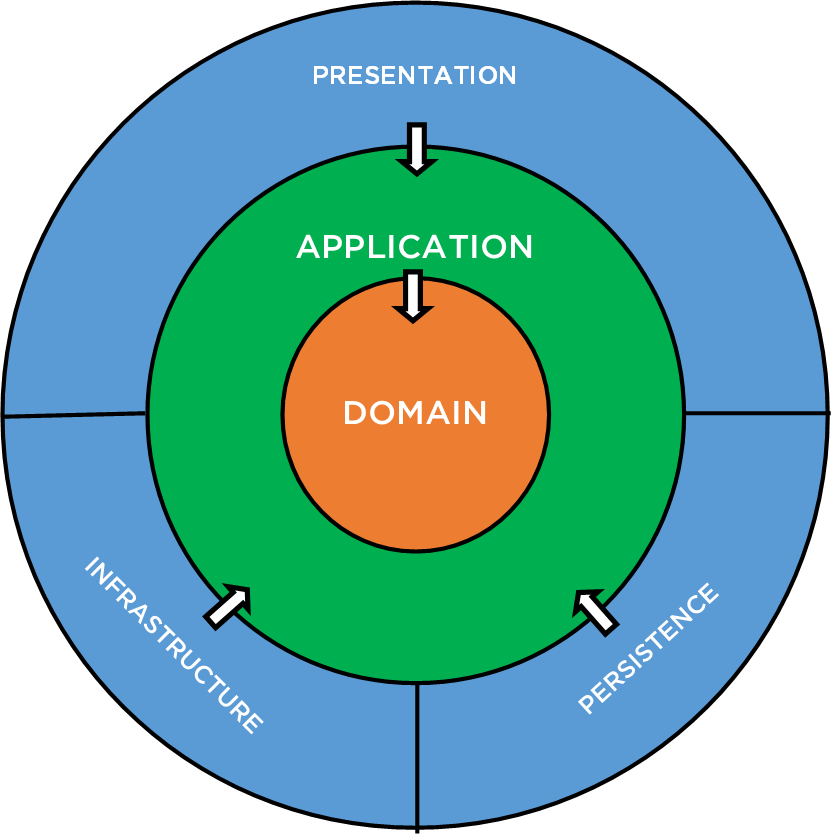
\includegraphics[width=\linewidth,height=\textheight,keepaspectratio]{CleanArchitecture.png}
\end{frame}
\begin{frame}
    \begin{description}[font=$\bullet$]
        \item Lösungen für die Probleme
              \begin{description}[font=$\bullet$]
                  \item Zeit + viele Google Suchen
              \end{description}
        \item Wer hat an der Bearbeitung teilgenommen?
              \begin{description}[font=$\bullet$]
                  \item Nick
                  \item Jonathan
                  \item Bruno
              \end{description}
    \end{description}
\end{frame}
\subsection{Deployment}
\begin{frame}
    \begin{description}[font=$\bullet$]
        \item Anwendung verwendet keine Microservice Architektur, da dies zusätzlicher Aufwand wäre
        \item Anwendung wird in Docker Containern deployed
        \item Zur Zeit sind 3 Container geplant. Datenbank (MS SQL Server), Backend (Asp.Net), Frontend(Nginx)
        \item Container werden mittels Docker Compose gestartet
    \end{description}
\end{frame}
\section{Tech Demo}
\begin{frame}
    \frametitle{Tech Demo}
\end{frame}



\end{document}


\end{document}